See Fig. \ref{fig:1.2.7}. Let the vertices be $\vec{A},\vec{B},\vec{C}$.
 The midpoints of each side are
\begin{align}
\vec{D} &= \frac{\vec{A}+\vec{B}}{2} = \myvec{0\\1} \\
\vec{E} &= \frac{\vec{B}+\vec{C}}{2} = \myvec{1\\0} \\
\vec{F} &= \frac{\vec{A}+\vec{C}}{2} = \myvec{1\\2} \\
\end{align}
 Area of a $\triangle$ ABC is given by 
\begin{multline}
 \frac{1}{2} \norm{\brak{\vec{E}-\vec{D}}\times\brak{\vec{F}-\vec{D}}}\\
= \frac{1}{2}\norm{\myvec{0\\-1} \times \myvec{1\\1}}
\\
= 1
\end{multline}

\begin{figure}[!ht]
\centering
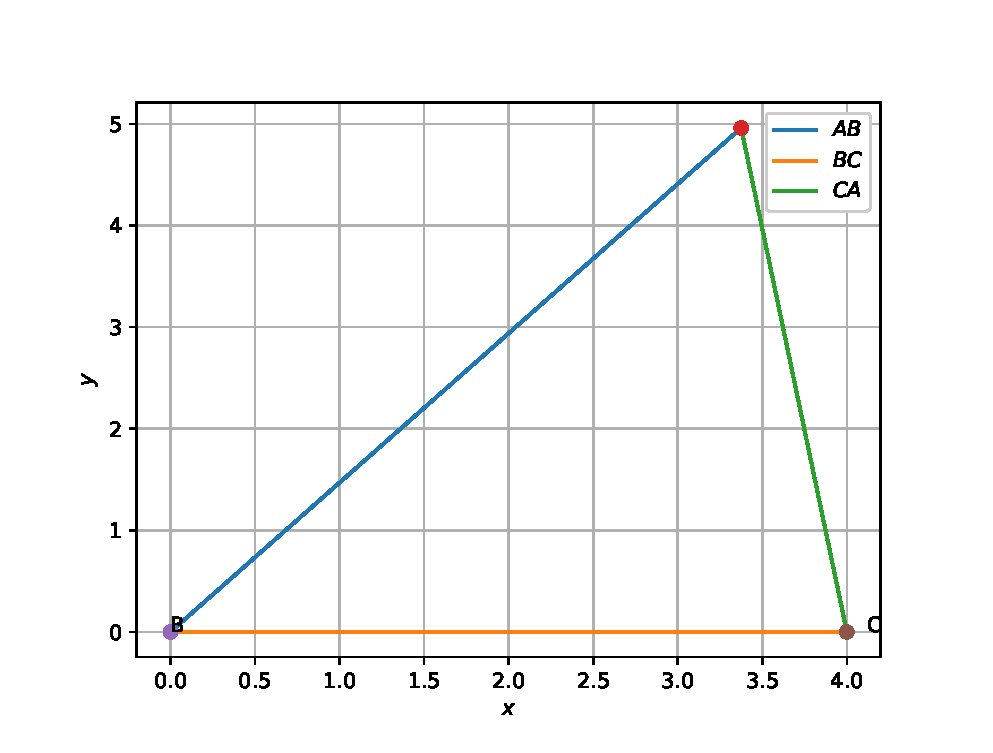
\includegraphics[width= \columnwidth]{./solutions/7/figs/triangle/triangle.eps}
\caption{}
\label{fig:1.2.7}
\end{figure}

 Download the python code for finding a triangle's area from
\begin{lstlisting}
solutions/7/codes/triangle/area_tri_area.py
\end{lstlisting}
and the figure from
\begin{lstlisting}
solutions/7/figs/triangle/draw_triangle.py
\end{lstlisting}

